\begin{abstract}

The coordinate systems and units used in \hisparc data and analysis are
illustrated and described. We also have to deal with other coordinate
systems such as the one used in \corsika and some used as intermediary
in coordinate transformations. The conversions and relations between
these systems are given.

\end{abstract}


\section{Introduction}

Since we have to work with many coordinate systems it can be hard to
keep track of the definitions of each. This document is meant as a
reference to easily find the relations between the different systems.
First coordinate systems used by \hisparc will be discussed. Including
the units that are used and where it is used. Then other coordinate
systems that we have to deal with are discussed, including ways to
convert from those to our usual coordinate systems.

Make sure that the angles are converted to the correct units for the
cosine and sine functions when converting between coordinate systems.
The use of radians or degrees depends on the programming language.


\section{Geographic}

Geographic coordinate systems define a point on the Earth. For \hisparc
three systems are used: WGS84, ECEF and ENU. \figref{fig:wgs84_ecef_enu}
illustrates the relationships between these systems. Additionally a
compass based system is used for detector locations relative to \gps
antenna. These systems are described in the following sections. The
conversion formulae are taken from \cite{wikipedia:2014aa}.

\begin{figure}
    \centering
    \tdplotsetmaincoords{70}{95}

\pgfmathsetmacro{\rvec}{.8}
\pgfmathsetmacro{\latitude}{90-45}  % phi
\pgfmathsetmacro{\longitude}{50}  % lambda

\begin{tikzpicture}[scale=5,thick,tdplot_main_coords]

    \definecolor{base}{RGB}{128,128,128}; % grey
    \definecolor{wgs84}{RGB}{255,153,0}; % orange
    \definecolor{ecef}{RGB}{13,98,153}; % blue
    \definecolor{enu}{RGB}{0,184,0}; % green

    \coordinate (O) at (0,0,0);

    % base
    \draw[base] (O) circle (\rvec);
    \draw[base] (\rvec,-.2,0) node[anchor=north east,rotate=-10] {Equator};
    \tdplotsetthetaplanecoords{90};
    \draw[base,tdplot_rotated_coords] (O) circle (\rvec);
    \tdplotsetthetaplanecoords{0};
    \draw[base,tdplot_rotated_coords] (\rvec,0,0) arc (0:90:\rvec)
        node[above right,rotate=88] {Prime Meridian};
    \tdplotsetthetaplanecoords{\longitude};
    \draw[base,dashed,tdplot_rotated_coords] (\rvec,0,0) arc (0:90:\rvec);

    % ECEF
    \draw[ecef,->,-stealth] (O) -- (1,0,0) node[anchor=north]{$X$};
    \draw[ecef,->,-stealth] (O) -- (0,1,0) node[anchor=west]{$Y$};
    \draw[ecef,->,-stealth] (O) -- (0,0,1) node[anchor=south]{$Z$};
    \tdplotsetcoord{P}{\rvec}{\latitude}{\longitude};
    \draw[->,-stealth] (O) -- (P);
    \draw[dashed] (O) -- (Pxy);
    \draw[dashed] (P) -- (Pxy);

    % WGS84
    \tdplotdrawarc[wgs84,->,-stealth]
        {(O)}{0.25}{0}{\longitude}{anchor=north}{$\lambda$};
    \tdplotsetthetaplanecoords{\longitude};
    \tdplotdrawarc[wgs84,->,-stealth,tdplot_rotated_coords]
        {(0,0,0)}{0.25}{90}{\latitude}{anchor=south west}{$\phi$};

    % ENU
    \tdplotsetrotatedcoords{\longitude}{\latitude}{0};
    \tdplotsetrotatedcoordsorigin{(P)};

%   This should be the ENU axes, but I cant find the correct rotation:
%    \draw[enu,tdplot_rotated_coords,->] (0,0,0) -- (.3,0,0) node[anchor=west]{$East$};
%    \draw[enu,tdplot_rotated_coords,->] (0,0,0) -- (0,.3,0) node[anchor=south]{$North$};
%    \draw[enu,tdplot_rotated_coords,->] (0,0,0) -- (0,0,.4) node[anchor=south]{$Up$};

    \draw[enu,->,-stealth,tdplot_rotated_coords] (0,0,0) -- (-.45,0,0)
        node[anchor=south]{$North$};
    \draw[enu,->,-stealth,tdplot_rotated_coords] (0,0,0) -- (0,.45,0)
        node[anchor=west]{$East$};
    \draw[enu,->,-stealth,tdplot_rotated_coords] (0,0,0) -- (0,0,.45)
        node[anchor=south]{$Up$};

\end{tikzpicture}

    \caption{Relationship between the WGS84 (orange), ECEF (blue) and ENU
             (green) coordinate systems. The Prime meridian is the IERS
             Reference Meridian.}
    \label{fig:wgs84_ecef_enu}
\end{figure}


\subsection{World Geodetic System 1984 (WGS84)}

The location of a \hisparc station is determined by means of a \gps
antenna (one antenna for each station). The \gps returns coordinates in
the WGS84 coordinate system. This defines a position with a latitude
($\phi$), longitude ($\lambda$) and altitude. The latitude and longitude
are defined in decimal degrees, the altitude in meters. Latitude is the
angular distance between a location and the equator, angles towards
north are positive. The longitude is the angular distance of a location
to the Reference Meridian (from now on referred to as the prime
meridian) defined by the International Earth Rotation and Reference
Systems Service (IERS), angles towards east are positive. The altitude
is the height above an ellipsoid that approximates the shape of the
Earth. The parameters which define this ellipsoid are given in
\eqref{eq:wgs84}.


\subsection{Earth-Centered, Earth-Fixed (ECEF)}

The ECEF coordinate system has its origin as the center of the Earth
(Earth-Centered), and its axes are aligned with the WGS84 system. The
z-axis points to North. The x-axis crosses the Earth surface where the
equator (\SI{0}{\degree} latitude) intersects the prime meridan
(\SI{0}{\degree} longitude). The y-axis intersects the equator at
\SI{90}{\degree} longitude. The axes rotate with the Earth
(Earth-Fixed). A position is defined by the $X$, $Y$, and $Z$
coordinates, each given in meters.

The formulae to convert WGS84 coordinates to ECEF coordinates are:

\begin{equation}
    \begin{array}{l}
        X = \left(N + \mathrm{altitude}\right) \cos{\phi} \cos{\lambda} \ , \\
        Y = \left(N + \mathrm{altitude}\right) \cos{\phi} \sin{\lambda} \ , \\
        Z = \left(\frac{b^2}{a^2} N + \mathrm{altitude}\right) \sin{\phi} \ . \\
    \end{array}
\end{equation}

\noindent
For the paramaters that define the ellipsoidal approximation of the
Earth surface we have

\begin{equation}
    \label{eq:wgs84}
    \begin{array}{l}
        a = \SI{6378137.0}{\meter} \ , \\
        f = \frac{1}{298.257223563} \ , \\
        b = a (1 - f) \ , \\
        e = \sqrt{2 f - f^2} \ , \\
        N = \frac{a}{\sqrt{1 - e^2 \sin{\phi}^2}} \ , \\
    \end{array}
\end{equation}

\noindent
here $a$ is the semi-major axis, $f$ the flattening, $b$ the semi-minor
axis and $e$ the eccentricity of the ellipsoid. $N$ is the Normal, which
is the distance from a location on the surface of the ellipsoid to the
intersection of the normal of the location and the z-axis.


\subsection{East, North, Up (ENU)}

East, North, Up is often used to obtain relative locations and angles
between locations. It is a local coordinate system in a plane tangential
to the WGS84 elipsoid. From the reference position the positive x-axis
(East) is in the eastern direction, the positive y-axis (North) is
towards north, and the positive z-axis (Up) is towards the Zenith. All
distances are in meters.

The formulae to convert ECEF to ENU with a given reference position are:

\begin{equation}
    \begin{bmatrix}
    x \\ y \\ z
    \end{bmatrix}
    =
    \begin{bmatrix}
                 -\sin(\lambda_r) &               \cos(\lambda_r) &           0. \\
    -\sin(\phi_r) \cos(\lambda_r) & -\sin(\phi_r) \sin(\lambda_r) & \cos(\phi_r) \\
     \cos(\phi_r) \cos(\lambda_r) &  \cos(\phi_r) \sin(\lambda_r) & \sin(\phi_r)
    \end{bmatrix}
    \begin{bmatrix}
    X - X_r \\ Y - Y_r \\ Z - Z_r
    \end{bmatrix}
\end{equation}

where  $(X, Y, Z)$ and $(x, y, z)$ are the location in ECEF and ENU
respectively. $(\phi_r, \lambda_r)$ and $(X_r, Y_r, Z_r)$ are the
reference position in WGS84 and ECEF respectively.


\subsection{Compass}

For reconstruction of events the precise location of the individual
detectors in a station is required. The location of detectors are taken
relative to the \gps antenna, because that position is known. We use a
system that requires a distance and angle measurement, see
\figref{fig:enu_compass}. The distance ($r$) between the \gps and a
detector (center of the scintillator) is measured (in meters), the angle
($\alpha$) relative to the North Pole is determined using a compass.
This angle is in degrees and goes from North to East (NESW). Note that
there is a difference between the magnetic and geographic north pole.
The difference can be up to \SI{3}{\degree} for some \hisparc station
locations \cite{canada:2013aa}. The rotation angle of the detector
itself ($\beta$) is defined as the angle of the long side of the
detector relative to the North Pole (positive towards East).

\begin{figure}
    \centering
    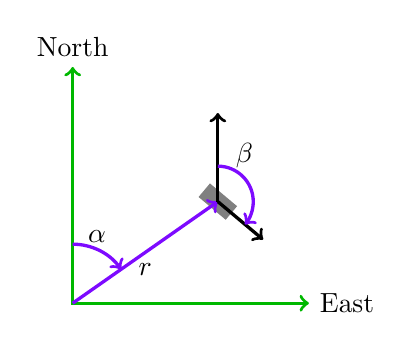
\begin{tikzpicture}[scale=1.5,line width=1.2pt]

  \definecolor{enu}{RGB}{0,184,0} % green
  \definecolor{compass}{RGB}{125,10,255} % purple
  \definecolor{base}{RGB}{128,128,128} % grey

  % Origin
  \coordinate (o) at (0,0);

  % Draw ENU axes
  \draw [enu,<->]
      (0,2) node[black] (yaxis) [above] {North} |-
      (2,0) node[black] (xaxis) [right] {East};

  % Draw a detectors
  \coordinate (d0) at (35:1.5);
  \fill[base,rotate=-40] (d0) ++(-.15,-.075) rectangle +(.3,.15);

  % Draw distance line
  \draw[compass,->] (o) -- node[black,below] {$r$} (d0);
  % Draw angle line
  \draw[compass,->] (0,.5) arc (90:35:.5);
  \draw[compass] (70:.6) node[black] {$\alpha$};

  % Draw North from detector
  \draw[->] (d0) -- +(0,.75);
  % Draw detector angle
  \draw[->] (d0) -- +(-40:.5);

  % Draw angle line
  \draw[compass,->] (d0) ++(0,.3) arc (90:-40:.3);
  \draw[compass] (d0) ++(60:.45) node[black] {$\beta$};

\end{tikzpicture}

    \caption{Relationship between the ENU (green) and Compass (purple)
             coordinate system and how it is used to define the position
             and rotation of a detector.}
    \label{fig:enu_compass}
\end{figure}

The formulae to convert the location of a station in Compass coordinates
to ENU are:

\begin{equation}
    \begin{array}{l}
        x = r * \sin{\alpha} \ , \\
        y = r * \cos{\alpha} \ , \\
        z = z \ . \\
    \end{array}
\end{equation}


\section{Time}

For \hisparc events it is important to know precisely when
they occur, a \gps is used to get synchronized and precise timing. This
gives us a timestamp, but this needs to be converted to other time
systems.


\subsection{\gps time}

\gps time started counting on 6 January 1980 00:00 UTC, i.e.
\num{315964800} UNIX seconds after the UNIX epoch of 1 January 1970
00:00 UTC. \gps time is a continuously increasing number. This is
different from UTC time in which certain seconds are repeated when `leap
seconds' are added. Currently the difference between UTC and \gps time
is 16 seconds. From the \hisparc electronics we get a \gps timestamp,
adjusted to the UNIX epoch. The timestamp is given in nanoseconds, i.e.
the number of nanoseconds that have passed since the UNIX epoch. The
\gps timestamp is a large number and requires 64-bits to represent the
number. For instance the \gps timestamp for 1 December 2014 at
00:00:29.886222166 (\gps time) is \num{1417392029886222166}.
\cite{usno:2012aa}.


\subsection{UTC time}

Similar to \gps but corrected with leap seconds to keep it more in sync
with solar time. A leap second means that a second is counted twice. The
IERS decides when to add leap seconds. \hisparc does not use UTC time
because of the duplicate timestamps, which makes it possible for a
station to detect two events at the `same time'. Moreover, it causes
issues when looking for coincidences between stations.


\subsubsection{Leap seconds}

Leap seconds can be introduced at the end of either 30 June or 31
December, the leap second is represented in UTC time as 23:59:60.
\tabref{table:leapseconds} gives a list of the recent leap seconds,
which are important for \hisparc. Leap seconds are announced about 6
months before they take effect.

\begin{table}
    \centering
    \begin{tabular}{ l | c }
        Date & Leap seconds \\
        \hline
        31 December, 1998 & 13 \\
        31 December, 2005 & 14 \\
        31 December, 2008 & 15 \\
        30 June, 2012 & 16 \\
        \hline
    \end{tabular}
   \caption{Leap seconds in effect or introduced after 2002. This is the
            amount of seconds that \gps time is ahead of UTC time.}
   \label{table:leapseconds}
\end{table}


\subsection{Julian Date (JD)}

Decimal number counting the number of days since 1 January 4713 B.C.
12:00:00. Calculating this is not trivial since one has to account for
the fact that the 5th up to and including the 14th of October in 1582 do
not exist. Those ten days were skipped because the Julian calendar,
which was used before that gap, introduced too many leap years, every
year divisible by 4 was a leap year. The Gregorian calendar used
afterwards compensated by having less leap years. Leap years still occur
when years are divisible by 4, except when they are also divisible by
100 (e.g. 1900), except when they are also divisible by 400 (e.g. 2000)
\cite{acf:2014aa}. Consider these examples: 1999 is not divisible by 4
so not a leap year, 2004 is divisible by 4 and not by 100 and is a leap
year, 1900 is divisible by 4 and 100 but not 400 so is not a leap year,
and 2000 is divisible by 4, 100 and 400 and is therefore a leap year.


\subsubsection{Modified Julian Date (MJD)}

Modified Julian Date to keep number shorter uses epoch 17 November 1858
00:00:00. The difference between a Modified Julian Date and a Julian
Date is 2400000.5 days. The .5 days moves the reference time from noon
to midnight.

\begin{equation}
    MJD = JD - 2400000.5
\end{equation}


\subsection{Sidereal Time}

In a solar day the Earth rotates more than \SI{360}{\degree} around its
axis because it orbits around the Sun, causing the position of the Sun
relative to the Earth to change. The Earth orbits the Sun every 365.25
days, so in one day the the orbit proceeds by
$\frac{\SI{360}{\degree}}{\SI{365.25}{\day}} \approx
\SI{1}{\degree\per\day}$. So an extra rotation of approximately
\SI{1}{\degree} around its axis is required to make the same part of the
Earth face the Sun (a solar day). In sidereal time the rotation of Earth
relative to the `fixed' background stars is taken. A sidereal day is a
full rotation of Earth around its axis, relative to background stars.
This is around \SI{4}{\minute} shorter than a solar day. In
\figref{fig:sidereal_time} the difference between a solar and sidereal
day is illustrated.

\begin{figure}
    \centering
    \pgfmathsetmacro{\rsun}{.2}
\pgfmathsetmacro{\rearth}{.15}
\pgfmathsetmacro{\AU}{1.1}
\pgfmathsetmacro{\margin}{.05}

\pgfmathsetmacro{\orbit}{270}
\pgfmathsetmacro{\siderealday}{32}
\pgfmathsetmacro{\solarday}{50}
\pgfmathsetmacro{\omargin}{10}

\begin{tikzpicture}[scale=2,thick]

    \definecolor{base}{RGB}{128,128,128}; % grey
    \definecolor{sidereal}{RGB}{44,92,198}; % blue
    \definecolor{solar}{RGB}{202,112,27}; % orange
    \definecolor{earth}{RGB}{0,184,0}; % green

    % coordinates
    \coordinate (O) at (0,0);
    \coordinate (earth_0) at (\orbit:\AU);
    \coordinate (earth_1) at (\orbit+\siderealday:\AU);
    \coordinate (earth_2) at (\orbit+\solarday:\AU);

    % Earth
    \draw[base,dashed] (O) circle (\AU);
    \draw[earth] (250:\AU) node[anchor=north east] {Earth};
    \draw[earth,fill=green] (earth_0) circle (\rearth);
    \draw[earth,fill=green] (earth_1) circle (\rearth);
    \draw[earth,fill=green] (earth_2) circle (\rearth);

    % AU
    \draw[base,dashed] (O) -- (earth_0);
    \draw[base,dashed] (O) -- (earth_1);
    \draw[base,dashed] (O) -- (earth_2);

    % Sun
    \draw[solar,fill=yellow] (O) circle (\rsun);
    \draw[solar] (180:\rsun) node[anchor=north east] {Sun};

    % Prime Meridian
    \draw (earth_0) -- ($ (earth_0)!\rearth!(O) $);
    \draw (earth_1) -- ++(90:\rearth);
    \draw (earth_2) -- ($ (earth_2)!\rearth!(O) $);

    % Earth orbit
    \tdplotdrawarc[base,-stealth]
        {(O)}{\AU-\margin}{\orbit+\omargin}{\orbit+\siderealday-\omargin}
        {}{};
    \tdplotdrawarc[sidereal,-stealth]
        {(O)}{\AU+\rearth+\margin+\margin}{\orbit}{\orbit+\siderealday}
        {anchor=north}{Sidereal day};
    \tdplotdrawarc[solar,-stealth]
        {(O)}{\AU+\rearth+\margin}{\orbit}{\orbit+\solarday}
        {anchor=north west}{Solar day};

    % Earth rotation
    \tdplotdrawarc[base,-stealth]
        {(earth_0)}{\rearth-\margin}{110}{430}{anchor=west}{};

    % Earth rotation
    \tdplotdrawarc[base] {(O)}{\rsun+\margin}{\orbit}{\orbit+\siderealday}{}{};
    \tdplotdrawarc[base] {(earth_1)}{\rearth+\margin}{90}{90+\siderealday}{}{};


    % Stellar background
    \draw[sidereal,->] ($ (O) + (90:\rsun+\margin) $) -- ++(90:.2)
        node[anchor=south] {Background stars};
    \draw[sidereal,->] ($ (earth_0) + (90:\rearth+\margin) $) -- ++(90:.2);
    \draw[sidereal,->] ($ (earth_1) + (90:\rearth+\margin) $) -- ++(90:.2);
    \draw[sidereal,->] ($ (earth_2) + (90:\rearth+\margin) $) -- ++(90:.2);

\end{tikzpicture}

    \caption{This shows the orbit of Earth (green) around the Sun
             (yellow). The black line on the Earth represents the prime
             meridian. A full rotation of the Earth causes the prime
             meridian to point to the same background stars, this is a
             sidereal day. It takes longer, due to the orbit of the
             Earth, for the prime meridian to point to the Sun again,
             which is a solar day. Used sizes and angles are
             illustrative, not realistic.}
    \label{fig:sidereal_time}
\end{figure}


\subsubsection{Greenwich Mean Sidereal Time (GMST)}

GMST is the hour angle of the vernal equinox (\secref{sec:celestial})
with respect to the prime meridian at Greenwich, expressed in decimal
hours \cite{kaplan:2011aa}. This is illustrated in
\figref{fig:wgs84_gmst_lst}.

\begin{equation}
    GMST = 6.697374558 + 0.06570982441908 D0 + 1.00273790935 H + 0.000026 T^2
\end{equation}

Here $D0$ is the Julian Date of the previous midnight using the J2000
epoch (1 January, 2000 12:00 UTC or Julian date 2451545.0), $H$ is the
number of hours since the last midnight, and $T$ is the number of
centuries since J2000.

\begin{figure}
    \centering
    \pgfmathsetmacro{\rlen}{1.5}
\pgfmathsetmacro{\longitude}{80}  % lambda
\pgfmathsetmacro{\gmst}{45}  % Greenwich mean sidereal time
\pgfmathsetmacro{\lst}{\gmst+\longitude}  % local sidereal time in degrees

\begin{tikzpicture}[scale=2,thick]

    \definecolor{base}{RGB}{128,128,128}; % grey
    \definecolor{wgs84}{RGB}{255,153,0}; % orange
    \definecolor{side}{RGB}{13,98,153}; % blue
    \definecolor{enu}{RGB}{0,184,0}; % green
    \definecolor{compass}{RGB}{125,10,255}; % purple
    \definecolor{equa}{RGB}{253,39,39}; % red
    \definecolor{time}{RGB}{15,171,135}; % teal

    \coordinate (O) at (0,0);

    % base
    \draw[base] (O) circle (\rlen); % Equator
    \tdplotdrawarc[base,->,-stealth]
        {(O)}{.2}{20}{340}{anchor=east}{Rotation};

    % Prime Meridian
    \draw[base] (O) -- (0:\rlen)
        node[right] {Prime Meridian};

    % WGS84
    % longitude
    \tdplotdrawarc[wgs84,->,-stealth]
        {(O)}{0.5}{0}{\longitude}{anchor=north}{$\lambda$};

    % gmst
    \tdplotdrawarc[time,->,-stealth]
        {(O)}{\rlen-.3}{-\gmst}{0}{anchor=south east}{GMST};
    \tdplotdrawarc[side,->,-stealth]
        {(O)}{\rlen-.2}{-\gmst}{\lst-\gmst}{anchor=east}{LST};

    % observer
    \draw[color=black,->,-stealth] (O) -- (\longitude:\rlen)
        node[above right] {Observer};

    % Equatorial
    \draw[base,->,-stealth] (O) -- (-\gmst:\rlen+.5)
        node[anchor=north]{$\vernal$};

\end{tikzpicture}

    \caption{Top-down view of Earth showing the relation between GMST
             (teal) and LST (blue) for an observer at a longitude
             $\lambda$ (orange). The observer and prime meridian move with
             the rotation of the Earth, the vernal equinox does not.}
    \label{fig:wgs84_gmst_lst}
\end{figure}


\subsubsection{Local Sidereal Time (LST)}

Similar to GMST but takes observers longitude into account.

To get the Local Sidereal Time the observers longitude has to be added
to the GMST. This is illustrated in \figref{fig:wgs84_gmst_lst}. Since
the longitude is given in degrees is has to be divided by 15 to get
hours, because $\frac{\SI{360}{\degree}}{\SI{24}{\hour}} =
\SI{15}{\degree\per\hour}$, so the equation becomes:

\begin{equation}
    \begin{array}{l}
        \mathit{LST} = \mathit{GMST} + \frac{\lambda}{15} \ . \\
    \end{array}
\end{equation}


\section{Celestial}
\label{sec:celestial}

Here we describe the different coordinate systems that are used to
define the direction (origin) of an air shower. The Zenith and Azimuth
and Horizontal systems rotate with the rotation of the Earth, because
they are linked to the location of the observer. The Equatorial system
is linked to the celestial sphere and independent from the rotation of
Earth. To transform from Zenith and Azimuth to Equatorial the position
of the observer and time of observation are also required.


\subsection{Zenith and Azimuth}

When a station detects a shower we try to reconstruct the direction of
its origin, i.e. the position on the sky the shower came from. This
direction is then given by a zenith and azimuth coordinate. These
coordinates define a point on the semi-sphere that is the sky above the
detection station. The Zenith is the point directly above the observer.
The zenith angle is the angle between the direction and the Zenith
point, so straight up is \SI{0}{\radian} and the horizon \SI{\pi /
2}{\radian}. The azimuth is the direction in the horizontal plane, it
starts at East (\SI{0}{\radian}) then goes to North (ENWS). This is
illustrated in pink in \figref{fig:enu_horizontal}.

We do not expect nor consider air showers from below the horizon, so the
zenith angles, defined in radians, are an angle in the range [0,
$\frac{\pi}{2}$). The azimuth is restricted to the range [$-\pi$, $\pi$).

\begin{figure}
    \centering
    \tdplotsetmaincoords{70}{-10}

\pgfmathsetmacro{\rlen}{.8}
\pgfmathsetmacro{\zenith}{90-45}  % theta
\pgfmathsetmacro{\azimuth}{300}  % phi

\begin{tikzpicture}[scale=5,thick,tdplot_main_coords]

    \definecolor{base}{RGB}{128,128,128}; % grey
    \definecolor{wgs84}{RGB}{255,153,0}; % orange
    \definecolor{ecef}{RGB}{13,98,153}; % blue
    \definecolor{enu}{RGB}{0,184,0}; % green
    \definecolor{zenazi}{RGB}{200,20,200}; % pink
    \definecolor{hori}{RGB}{200,180,20}; % gold

    % coordinates
    \coordinate (O) at (0,0,0);
    \tdplotsetcoord{P}{\rlen}{\zenith}{\azimuth};

    % base
    \draw[base] (O) circle (\rlen);
    \draw[base] (-\rlen*.8,-\rlen*.8,0) node[anchor=west,rotate=-10] {Horizon};
    \tdplotsetthetaplanecoords{\azimuth};
    \draw[base,dashed,tdplot_rotated_coords] (\rlen,0,0) arc (0:90:\rlen);
    \draw[base,dashed,tdplot_rotated_coords] (0,0,0) -- (0,\rlen,0);
%    \draw[base,dashed] (P) -- (Pxy);

    % ENU
    \draw[enu,-stealth] (O) -- (1,0,0) node[anchor=west]{East};
    \draw[enu,-stealth] (O) -- (0,1,0) node[anchor=south east]{North};

    % Zenith Azimuth
    \tdplotdrawarc[zenazi,-stealth]
        {(O)}{0.2}{0}{\azimuth}{anchor=south east}{$\phi$};

    % Horizontal
    \tdplotdrawarc[hori,-stealth]
        {(O)}{0.4}{90}{\azimuth-360}{anchor=south west}{$A$};

    \tdplotsetthetaplanecoords{\azimuth};
    % Zenith Azimuth
    \tdplotdrawarc[zenazi,-stealth,tdplot_rotated_coords]
        {(0,0,0)}{0.25}{0}{\zenith}{anchor=south west}{$\theta$};
    % Horizontal
    \tdplotdrawarc[hori,-stealth,tdplot_rotated_coords]
        {(0,0,0)}{0.25}{90}{\zenith}{anchor=south west}{$a$};

    % ENU
    \draw[enu,-stealth] (O) -- (0,0,1) node[anchor=south]{Up};

    % star
    \draw[-stealth] (O) -- (P) node[anchor=south west] {$\star$};

\end{tikzpicture}

    \caption{Relationship between the ENU (green), Zenith Azimuth (pink)
             and horizontal (gold) coordinate systems.}
    \label{fig:enu_horizontal}
\end{figure}


\subsection{Horizontal}

This is a system used as intermediary for some coordinate conversions.
It uses azimuth ($A$) and altitude ($a$) to define a direction. The
altitude is the opposite of the zenith, so \SI{0}{\radian} is horizontal
and \SI{\pi / 2}{\radian} is the zenith. The azimuth definition also
differs, in Horizontal coordinates it moves from North to East (NESW).
This is illustrated in gold in \figref{fig:enu_horizontal}.

The formulae to convert from zenith ($\theta$) and azimuth ($\phi$) to
altitude ($a$) and azimuth ($A$) are:

\begin{equation}
    \begin{array}{l}
        a = \frac{\pi}{2} - \theta \ , \\
        A = \frac{\pi}{2} - \phi \ . \\
    \end{array}
\end{equation}


\subsection{Equatorial (J2000)}

\figref{fig:equatorial} shows the relation between the celestial sphere
and Equatorial coordinates. The right ascension ($\alpha$) is the angle
between the projection of the sky position ($\star$) on the plane of the
Celestial equator and the vernal equinox ($\vernal$). The declination
($\delta$) is the angle between the plane of the Celestial equator and
the sky position. Due to precession (change of the rotational axis) the
celestial positions slowly change over time, to compensate coordinates
are calculated as they would have been on a specific date, the J2000
epoch is commonly used. The equatorial coordinates are fixed to the
celestial sphere and not influenced by the rotation of the Earth.

\begin{figure}
    \centering
    \tdplotsetmaincoords{70}{95}

\pgfmathsetmacro{\rlen}{.4}

\pgfmathsetmacro{\clen}{1.6}
\pgfmathsetmacro{\ra}{50}  % right ascension in degrees
\pgfmathsetmacro{\dec}{90-50}  % declination in degrees

\begin{tikzpicture}[scale=3,thick,tdplot_main_coords]

    \definecolor{base}{RGB}{128,128,128}; % grey
    \definecolor{wgs84}{RGB}{255,153,0}; % orange
    \definecolor{ecef}{RGB}{13,98,153}; % blue
    \definecolor{enu}{RGB}{0,184,0}; % green
    \definecolor{compass}{RGB}{125,10,255}; % purple
    \definecolor{equa}{RGB}{253,39,39}; % red
    \definecolor{time}{RGB}{15,171,135}; % teal

    \coordinate (O) at (0,0,0);
    \coordinate (top) at (0,0,\rlen);

    % base
    \draw[base] (O) circle (\rlen);
    \draw[base] (\rlen,-.2,0);  % Equator
    \tdplotdrawarc[time,->,-stealth]
        {(0,0,\rlen)}{.2}{20}{340}{anchor=west}{};

    \tdplotsetthetaplanecoords{90};
    \draw[base,tdplot_rotated_coords] (O) circle (\rlen);

    % celestial base
    \draw[base] (O) circle (\clen);
    \draw[base] (\clen,-.75,0)
        node[anchor=north,rotate=-10] {Celestial Equator};
    \draw[base,->,-stealth] (O) -- (0,0,\clen + .3)
        node[anchor=south] {Celestial North Pole};
    \tdplotsetthetaplanecoords{90};
    \draw[base,tdplot_rotated_coords] (O) circle (\clen);

    % Equatorial
    \draw[base,->,-stealth] (O) -- (\clen + .3,0,0)
        node[anchor=north]{$\vernal$};

    \tdplotsetcoord{S}{\clen}{\dec}{\ra};
    \draw[->,-stealth] (O) -- (S) node[anchor=south west] {$\star$};

    \tdplotsetthetaplanecoords{\ra};
    \draw[base,dashed,tdplot_rotated_coords] (\clen,0,0) arc (0:90:\clen);
    \draw[base,dashed,tdplot_rotated_coords] (0,0,0) -- (0,\clen,0);
    \tdplotdrawarc[equa,->,-stealth,tdplot_rotated_coords]
        {(0,0,0)}{\clen}{90}{\dec}{anchor=west}{$\delta$};
    \tdplotdrawarc[equa,->,-stealth]
        {(O)}{\clen}{0}{\ra}{anchor=north}{$\alpha$};

\end{tikzpicture}

    \caption{This figures shows the relation between a position on the
             sky (black), Equatorial coordinates (red), and the
             Celestial sphere.}
    \label{fig:equatorial}
\end{figure}

Given an observers position in WGS84, a time of observation in LST and
horizontal coordinates pointing to the source the following formulae can
be used to get the corresponding equatorial coordinates \cite[p.
37]{duffet-smith:1990aa}.

\begin{equation}
    \begin{array}{l}
        \delta = \arcsin{\left((\sin{a} \sin{\phi}) +
                               (\cos{a} \cos{\phi} \cos{A})\right)} \ , \\
        \mathit{HA} = \arccos{\left(\frac{\sin{a} - (\sin{\phi} \sin{\delta})}
                                         {\cos{\phi} \cos{\delta}}\right)} \ , \\
        \alpha = \mathit{LST} - \mathit{HA} \ . \\
    \end{array}
\end{equation}

The output range of $\arccos$ is [0, $\pi$), while that of $\mathit{HA}$ is
[0, $2\pi$). If the azimuth is positive use: $\mathit{HA} = 2 \pi -
\mathit{HA}$.

Where $\phi$ the geographical latitude, $a$ the altitude, $A$ the
azimuth, $\mathit{LST}$ the Local sidereal time, $\delta$ is the
declination, $\alpha$ the right ascension and the intermediate variable
$\mathit{HA}$ is the hour angle. This is illustrated in
\figref{fig:wgs84_zenazi_lst_equatorial}.


\begin{figure}
    \centering
    \tdplotsetmaincoords{70}{95}

\pgfmathsetmacro{\rlen}{1.2}
\pgfmathsetmacro{\latitude}{90-35}  % phi
\pgfmathsetmacro{\longitude}{100}  % lambda

\pgfmathsetmacro{\clen}{3}
\pgfmathsetmacro{\ra}{28}  % right ascension in degrees
\pgfmathsetmacro{\dec}{90-50}  % declination in degrees

\pgfmathsetmacro{\gmst}{-45}  % Greenwich mean sidereal time
\pgfmathsetmacro{\lst}{\longitude+\gmst}  % local sidereal time in degrees

%\pgfmathsetmacro{\zenith}{22}  % theta
%\pgfmathsetmacro{\azimuth}{0}  % phi

\begin{tikzpicture}[scale=2,thick,tdplot_main_coords]

    \definecolor{base}{RGB}{128,128,128}; % grey
    \definecolor{wgs84}{RGB}{255,153,0}; % orange
    \definecolor{ecef}{RGB}{13,98,153}; % blue
    \definecolor{enu}{RGB}{0,184,0}; % green
    \definecolor{compass}{RGB}{125,10,255}; % purple
    \definecolor{equa}{RGB}{253,39,39}; % red
    \definecolor{time}{RGB}{15,171,135}; % teal
    \definecolor{zenazi}{RGB}{200,20,200}; % pink

    \coordinate (O) at (0,0,0);

    % base
    \draw[base] (O) circle (\rlen);
    \draw[base] (\rlen,-.2,0);  % Equator
    \tdplotsetthetaplanecoords{90};
    \draw[base,tdplot_rotated_coords] (O) circle (\rlen);
    \tdplotsetthetaplanecoords{\gmst};
    % Prime Meridian
    \draw[base,dashed,tdplot_rotated_coords] (0,0,0) -- (0,\rlen,0);
    \draw[base,tdplot_rotated_coords] (\rlen,0,0) arc (0:90:\rlen);
    \tdplotsetthetaplanecoords{\lst};
    \draw[base,dashed,tdplot_rotated_coords] (\rlen,0,0) arc (0:90:\rlen);
    \draw[base,dashed,tdplot_rotated_coords] (\clen,0,0) arc (0:90:\clen);
    \draw[base,dashed,tdplot_rotated_coords] (0,0,0) -- (0,\clen,0);

    \tdplotdrawarc[time,-stealth]
        {(0,0,\rlen)}{.2}{20}{340}{anchor=west}{};

    % celestial base
    \draw[base] (O) circle (\clen);
    \draw[base] (\clen,-.8,0)
        node[anchor=north east,rotate=-10] {Celestial Equator};
    \draw[base,-stealth] (O) -- (0,0,\clen + .3)
        node[anchor=south] {Celestial North Pole};
    \tdplotsetthetaplanecoords{90};
    \draw[base,tdplot_rotated_coords] (O) circle (\clen);

    % ECEF
%    \tdplotsetrotatedcoords{0}{0}{\gmst};
%    \draw[ecef,-stealth,tdplot_rotated_coords] (O) -- (\rlen+.2,0,0)
%        node[anchor=north] {$X$};
%    \draw[ecef,-stealth,tdplot_rotated_coords] (O) -- (0,\rlen+.2,0)
%        node[anchor=west] {$Y$};
%    \draw[ecef,-stealth,tdplot_rotated_coords] (O) -- (0,0,\rlen+.2)
%        node[anchor=west] {$Z$};

    % WGS84
    % longitude
    \tdplotsetrotatedcoords{0}{0}{\gmst};
    \tdplotdrawarc[wgs84,-stealth,tdplot_rotated_coords]
        {(O)}{0.4}{0}{\longitude}{anchor=north}{$\lambda$};
    % latitude
    \tdplotsetthetaplanecoords{\lst};
    \tdplotdrawarc[wgs84,-stealth,tdplot_rotated_coords]
        {(0,0,0)}{0.4}{90}{\latitude}{anchor=west}{$\phi$};

    % gmst
    \tdplotsetthetaplanecoords{\lst};
    \tdplotdrawarc[time,-stealth]
        {(O)}{\clen}{\lst}{\ra}{anchor=north west}{HA}; %  Flip arrow to other side?
    \tdplotdrawarc[time,-stealth]
        {(O)}{\rlen}{0}{\lst}{anchor=north}{LST};

    % observer
    \tdplotsetcoord{P}{\rlen}{\latitude}{\lst};
    \tdplotsetcoord{P'}{\clen}{\latitude}{\lst};
    \draw[color=black,-stealth] (O) -- (P);
    \draw[base] (P) -- (P') node[anchor=south west] {Zenith};
%    \draw[base,dashed] (P) -- (Pxy);

    % Equatorial
    \draw[base,-stealth] (O) -- (\clen + .3,0,0)
        node[anchor=north]{$\vernal$};

    \tdplotsetcoord{S}{\clen}{\dec}{\ra};
    \draw[-stealth] (O) -- (S) node[anchor=south west] {$\star$};
%    \draw[base,dashed] (S) -- (Sxy);


    % Observer to Star
    \tdplotsetrotatedcoords{\lst}{\latitude}{0};
    \tdplotsetrotatedcoordsorigin{(P)};

    \tdplotdrawarc[zenazi,-stealth,tdplot_rotated_coords]
        {(0,0,0)}{0.2}{90}{225}{anchor=south east}{$\phi$};
%    \tdplotsetthetaplanecoords{\ra};
%    \tdplotdrawarc[zenazi,-stealth,tdplot_rotated_coords]
%        {(0,0,0)}{0.2}{90}{240}{anchor=west}{$\phi$};

    \draw[base,tdplot_rotated_coords] (0,0,0) circle (.25);       
    \draw[color=black,-stealth] (P) -- (S);
%    \draw[enu,-stealth,tdplot_rotated_coords] (0,0,0) -- (-.5,0,0)
%        node[anchor=south]{N};
    \draw[enu,-stealth,tdplot_rotated_coords] (0,0,0) -- (0,.75,0)
        node[anchor=west]{E};
%    \draw[enu,-stealth,tdplot_rotated_coords] (0,0,0) -- (0,0,.35)
%        node[anchor=north west]{U};

    \tdplotsetrotatedthetaplanecoords{225};
    \tdplotdrawarc[zenazi,-stealth,tdplot_rotated_coords]
        {(0,0,0)}{0.8}{0}{40}{anchor=south west}{$\theta$};
    \draw[base,dashed,tdplot_rotated_coords] (0,0,0) -- (0,0.55,0);


    \tdplotsetrotatedcoordsorigin{(O)};
    \tdplotsetthetaplanecoords{\ra};
    \draw[base,dashed,tdplot_rotated_coords] (\clen,0,0) arc (0:90:\clen);
    \draw[base,dashed,tdplot_rotated_coords] (0,0,0) -- (0,\clen,0);
    \tdplotdrawarc[equa,-stealth,tdplot_rotated_coords]
        {(0,0,0)}{\clen}{90}{\dec}{anchor=west}{$\delta$};
    \tdplotdrawarc[equa,-stealth]
        {(O)}{\clen}{0}{\ra}{anchor=north}{$\alpha$};


\end{tikzpicture}

    \caption{Relationship between the WGS84 (orange), ENU (green),
             Zenith azimuth (pink), and clock (teal) and Equatorial
             (red) coordinate systems. $\vernal$ points to the vernal
             equinox, the point where the ecliptic and celestial equator
             cross in the Aries zodiac. WGS84 defines the position of
             the observer, LST defines the time of observation, ENU is
             the local coordinate system (only East is shown because it
             is used for the azimuth), and zenith and azimuth give the
             direction of shower origin. Combined these give the same
             position on the sky as the equatorial coordinates.}
    \label{fig:wgs84_zenazi_lst_equatorial}
\end{figure}


\section{\corsika}

\corsika is an extensive air shower simulation program which we use. It
uses coordinate systems which are slightly different from the ones we
employ \cite{heck:2013aa}.

\begin{figure}
    \centering
    \tdplotsetmaincoords{70}{-10}

\pgfmathsetmacro{\rlen}{.8}
\pgfmathsetmacro{\zenith}{90-45}  % theta
\pgfmathsetmacro{\azimuth}{40}  % phi

\begin{tikzpicture}[scale=5,thick,tdplot_main_coords]

    \definecolor{base}{RGB}{128,128,128}; % grey
    \definecolor{wgs84}{RGB}{255,153,0}; % orange
    \definecolor{ecef}{RGB}{13,98,153}; % blue
    \definecolor{enu}{RGB}{0,184,0}; % green
    \definecolor{hori}{RGB}{200,20,200}; % pink
    \definecolor{corsika}{RGB}{151,115,0}; % brown

    % coordinates
    \coordinate (O) at (0,0,0);
    \tdplotsetcoord{P}{\rlen}{\zenith}{\azimuth};
    \tdplotsetcoord{P'}{\rlen}{180-\zenith}{180 + \azimuth};

    % base
    \draw[base] (O) circle (\rlen);
    \draw[base] (-\rlen*.8,-\rlen*.8,0) node[anchor=west,rotate=-10] {};
    \tdplotsetthetaplanecoords{\azimuth};
    \draw[base,dashed,tdplot_rotated_coords] (\rlen,0,0) arc (0:90:\rlen);
    \draw[base,dashed] (P) -- (Pxy);
    \draw[base,dashed] (P') -- (P'xy);
    \draw[base,dashed,tdplot_rotated_coords] (0,-\rlen,0) -- (0,\rlen,0);

    % Horizontal
    \tdplotdrawarc[hori,-stealth]
        {(O)}{0.3}{0}{\azimuth}{anchor=west}{$\phi$};
    \tdplotsetthetaplanecoords{\azimuth};
    \tdplotdrawarc[hori,-stealth,tdplot_rotated_coords]
        {(0,0,0)}{0.2}{0}{\zenith}{anchor=south}{$\theta$};

    % ENU
    \draw[enu,-stealth] (O) -- (1,0,0) node[anchor=west]{East};
    \draw[enu,-stealth] (O) -- (0,1,0) node[anchor=south east]{North};
    \draw[enu,-stealth] (O) -- (0,0,1) node[anchor=south east]{Up};

    % CORSIKA
    \tdplotdrawarc[corsika,-stealth]
        {(O)}{0.3}{90}{\azimuth+180}{anchor=south}{$\Phi$};
    \tdplotsetthetaplanecoords{\azimuth};
    \tdplotsetrotatedcoordsorigin{(P)};
    \tdplotdrawarc[corsika,-stealth,tdplot_rotated_coords]
        {(0,0,0)}{0.2}{180}{180+\zenith}{anchor=north}{$\Theta$};

    \draw[corsika,->,dashed,-stealth] (O) -- (-1,0,0) node[anchor=east]{$y$};
    \draw[corsika,->,dashed,-stealth] (O) -- (0,1,0) node[anchor=south west]{$x$};
    \draw[corsika,->,dashed,-stealth] (O) -- (0,0,1) node[anchor=south west]{$z$};

    % star
    \draw[-stealth] (O) -- (P) node[anchor=south west] {$\star$};
    \draw[base,-stealth] (O) -- (P');

\end{tikzpicture}

    \caption{Relationship between the ENU (green), Zenith Azimuth (pink),
             and \corsika (brown) coordinates.}
    \label{fig:enu_corsika}
\end{figure}


\subsection{Geographic}

\corsika defines positions on the ground (or observation level) relative
to the point where the shower axis intersects the observation level.
Positive x axis points to magnetic North, positive y axis to the West,
and the z axis upwards. This is shown by the dashed brown lines in
\figref{fig:enu_corsika}.

The formulae to convert \corsika to ENU are:

\begin{equation}
    \begin{array}{l}
        x_{\mathrm{ENU}} = -y_{\mathrm{CORSIKA}} \ , \\
        y_{\mathrm{ENU}} = x_{\mathrm{CORSIKA}} \ , \\
        z_{\mathrm{ENU}} = z_{\mathrm{CORSIKA}} \ . \\
    \end{array}
\end{equation}


\subsection{Celestial}

\corsika looks from the point of view of the shower, so not the
direction it came form, but the direction it goes to. The $\Theta$ angle
is defined the same as our definition of zenith ($\theta$),
\SI{0}{\radian} is a shower from the zenith and \SI{\pi / 2}{\radian} is
a horizontal shower. The $\Phi$ angle is defined differently than our
definition of azimuth ($\phi$). First is the angle the shower is heading
towards and secondly a different reference is used. \SI{0}{\radian} is a
shower heading towards North, so coming from South, which we would
define as \SI{-\pi / 2}{\radian}. The (positive) rotation of the angle
is in the same direction, from North to West. This is shown by the brown
arced lines in \figref{fig:enu_corsika}.

The formulae to convert the \corsika direction to our azimuth and zenith
are:

\begin{equation}
    \begin{array}{l}
        \theta = \Theta \ , \\
        \phi = \Phi - \frac{\pi}{2} \ . \\
    \end{array}
\end{equation}

\section{Acknowledgements}

We want to thank Dr. J.J.M. Steijger for his careful checking of our methods. 
